
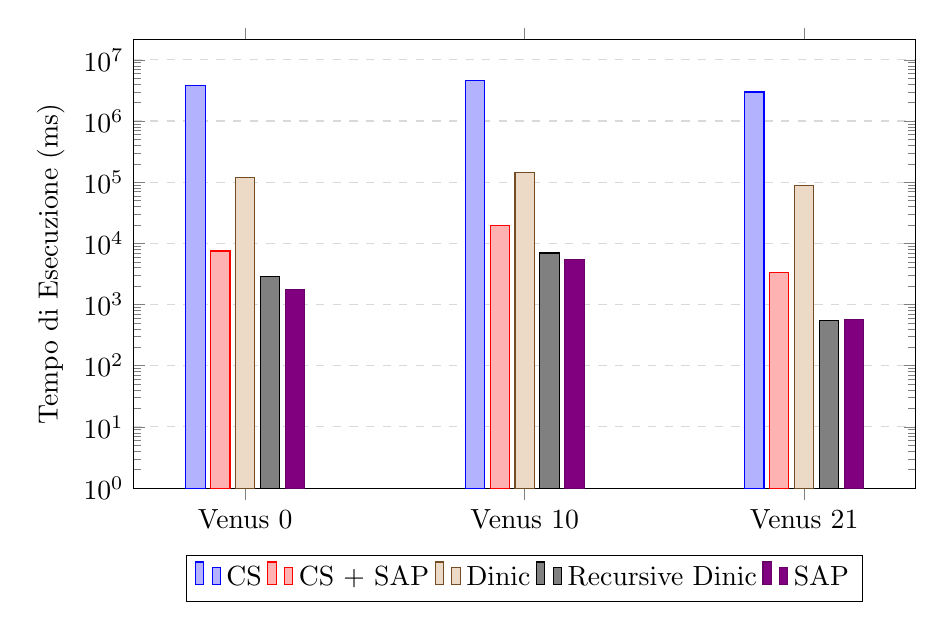
\begin{tikzpicture}
    \begin{semilogyaxis}[
        ybar,
        width=0.95\textwidth,
        height=0.6\textwidth,
        ylabel={Tempo di Esecuzione (ms)},
        symbolic x coords={Venus 0,Venus 10,Venus 21},
        xtick=data,
        point meta=y,
        legend style={at={(0.5,-0.15)}, anchor=north, legend columns=-1},
        ymajorgrids=true,
        grid style={dashed, gray!30},
        ymin=1,
        bar width=7pt,
        enlarge x limits=0.2
    ]
    \addplot coordinates {
        (Venus 0, 3750051.34)
        (Venus 10, 4597135.92)
        (Venus 21, 2985202.47)
    };
    \addlegendentry{CS}
    \addplot coordinates {
        (Venus 0, 7495.03)
        (Venus 10, 19600.23)
        (Venus 21, 3288.18)
    };
    \addlegendentry{CS + SAP}
    \addplot coordinates {
        (Venus 0, 118250.72)
        (Venus 10, 143449.83)
        (Venus 21, 89301.16)
    };
    \addlegendentry{Dinic}
    \addplot coordinates {
        (Venus 0, 2867.96)
        (Venus 10, 6963.97)
        (Venus 21, 550.24)
    };
    \addlegendentry{Recursive Dinic}
    \addplot coordinates {
        (Venus 0, 1773.21)
        (Venus 10, 5451.56)
        (Venus 21, 567.23)
    };
    \addlegendentry{SAP}

    \end{semilogyaxis}
\end{tikzpicture}
